\documentclass{standalone}

\usepackage{circuitikz}

\begin{document}

% INT_AY20_MP1_L05_Fig01-Arrow_attributes.png

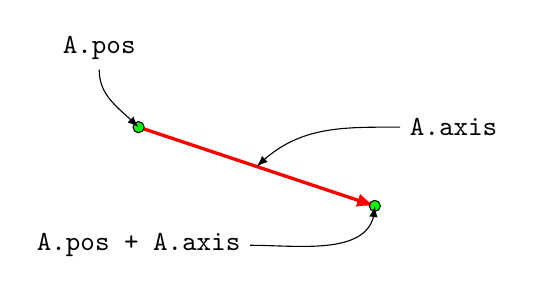
\begin{tikzpicture}[> = latex]

	% Vector + tail label and point
	
	\draw [->, red, very thick] (0, 0) coordinate (tail) -- coordinate [midway] (mid) (3, -1) coordinate (tip);
	
	\draw [fill = green] (tail) circle (2 pt);
	
	\node (pos) at (-0.5, 1) {\texttt{A.pos}};
	\draw [->] (pos.south) to [out = 270, in = 135] (tail);
	
	% Axis label
	
	\node (axis) at (4, 0) {\texttt{A.axis}};
	\draw [->] (axis.west) to [out = 180, in = 45] (mid);
	
	% Tip position label and point
	
	\draw [fill = green] (tip) circle (2 pt);

	\node (sum) at (0, -1.5) {\texttt{A.pos + A.axis}};
	\draw [->] (sum.east) to [out = 0, in = 270] (tip);
	
\end{tikzpicture}

\end{document}